\documentclass[11pt,a4paper]{article}
\usepackage[utf8x]{inputenc}
\usepackage[T1]{fontenc}
\usepackage{mathptmx} % Use Times Font
%\usepackage{listings}
\usepackage{amsmath}
\usepackage{amssymb}
\usepackage{tikz-cd}
\usepackage{enumerate}
%\usepackage{mathtools}
%\usepackage{theoremref}
\usepackage{amsthm}
\newcounter{thm}
\numberwithin{thm}{section}
\newtheorem{theorem}{Theorem}[thm]
\newtheorem{corollary}{Corollary}[thm]
\newtheorem{lemma}[thm]{Lemma}
\newtheorem{prop}[thm]{Proposition}
\newtheorem{remark}[thm]{Remark}
\newtheorem{definition}[thm]{Definition}
\newtheorem{example}[thm]{Example}

\newcommand{\dsum}{\bigoplus}
\newcommand{\iso}{\cong}
\newcommand{\defn}[1]{\textit{#1}}
\newcommand{\cat}[1]{\mathcal{#1}}
\newcommand{\RP}[1]{\mathbb{RP}^{#1}}
\newcommand{\CP}[1]{\mathbb{CP}^{#1}}
\newcommand{\S}[1]{\mathbb{S}^{#1}}

\title{Homology Theory and the Borsuk-Ulam Theorem}
\author{Malthe Sporring}

\begin{document}
\maketitle

\section{Notes and acknowledgements}
This text provides an introduction to homology theory from an axiomatic point of view. The reader is assumed to have knowledge of undergraduate level Algebra and Algebraic Topology, particularly \textit{groups, homotopies, homotopy equivalences} and \textit{quotient spaces}.

I am very grateful to Clark Barwick for supervising this project and for sharing both his knowledge and passion for the subject. I also wish to extend my gratitude to the University of Edinburgh School of Mathematics Vacation Scholarship and College Vacation Scholarship funds for funding this project.
\newpage
\section{Introduction}
One of the goals of algebraic topology is classifying spaces up to some definition of equivalence, typically homotopy equivalence. Establishing equivalence can be tedious, as it often requires the construction of an explicit homotopy equivalence. However, \textit{inequivalence} is often easier to establish by calculating \defn{homotopy invariants}. These are properties of a space that are preserved by homotopy equivalences, hence if two spaces have different invariants, they cannot be homotopy equivalent. One of the first major homotopy invariances the undergraduate student encounters are the homotopy groups $\pi_n(X),n\in \mathbb{N}\cup \{0\}$: the groups of maps $f:S^{n}\rightarrow X$ with some base point. The homotopy groups carry a lot of geometric information, but are notoriously difficult to compute. Even for a simple space like the $2$-sphere $S^2$, it is not obvious that there are non-trivial maps $S^3\rightarrow S^2$ (we show that such a map exists in section \ref{sec-complex-projective-space}), and it is even less obvious what the higher homotopy groups are. The groups $\pi_n(S^2)$ do not seem to follow a pattern, and remain an active area of research. Only recently in 2015 was it proven that $\pi_n(S^2)$ is not zero for all $n\geq 2$ \cite{Ivanov}.

To avoid these complications, we would like to find homotopy invariances that are easier to compute, and ideally, not at the cost of too much geometric information. The homology groups $H_n(X)$ are an example of such a homotopy invariant. Like the homotopy groups, they are a sequence of groups, one for each $n\in \mathbb{Z}$, but they are much simpler and easier to compute. For example, the spheres have the simple structure $$H_n(S^m)=\begin{cases}\mathbb{Z} & n=0,m\\ 0 & \text{otherwise}\end{cases}$$
Part of the reason why they are easier to compute is that they come with extra structure, most importantly a \defn{long exact sequence}, which, broadly speaking, relates the homology groups $H_nX$ to each other and to the homology groups $H_nA$ of a subspace $A\subseteq X$. Therefore, the more you know about some of the homology groups of a space and a subspace, the easier it is to calculate the rest.

Historically, homology groups were produced from a number of geometric methods. It was Eilenberg and Steenrod who united the different homology theories by laying out a set of axioms that all homology theories satisfy \ref{Eilenberg}. In this text, we will take such an axiomatic approach, proving all results directly from the axioms. In some ways this approach more directly shows the point of homology theory. As will become clear, we will very rarely want for the geometric construction, and in fact all (ordinary) homology theories which satisfy the same Eilenberg-Steenrod axioms and initial conditions are equivalent; the geometric construction contributes no more than can be captured in the axioms (REFERENCE). It is therefore believable that the main role of a geometric construction of homology theory is to prove the Eilenberg-Steenrod Axioms for that theory. For the results to be true we have to take given that there exists at least one homology theory which satisfies the axioms. Proving this is a major undertaking worth its own project. Singular Homology is an example of a homology theory which satisfies our assumptions, and the reader is invited to confirm that it satisfies the axioms in \cite{Hatcher}.

Homology theory is best understood in the language of category theory and chain complexes, which sections \ref{sec-category-theory} and \ref{sec-chain-complexes} are devoted to. In section \ref{sec-axioms}, we lay out the Eilenberg-Steenrod axioms and prove some immediate results for a general ordinary homology theory, most importantly the homology groups of the $n$-sphere. In the following sections we make the choice $H_0 \cdot=\mathbb{Z}$, which corresponds to Singular Homology. In sections \ref{sec-Mayer-Vietoris}, \ref{sec-degree-maps} and \ref{sec-cellular-homology} we lay out three practical methods for calculating homology groups; The Mayer-Vietoris Sequence, degree maps and Cellular Homology, and use them to prove some fascinating results.
\section{Chain Complexes}\label{sec-chain-complexes}
\begin{definition}
A \defn{chain complex} is a family $(A_i)_{i\in\mathbb{Z}}$ of abelian groups, as well as a family $(f_i:A_i\rightarrow A_{i+1})_{i\in \mathbb{Z}}$ of homomorphisms between consecutive groups, such that $im(f_i)\subset ker(f_{i+1})$. If we have equality instead of inclusion, the family is called an \defn{exact sequence}.
\end{definition}

We distinguish between \defn{short} and \defn{long exact sequences}, where short exact sequences are sequences with three or fewer consecutive non-zero groups, i.e. sequences of the form

% https://tikzcd.yichuanshen.de/#N4Igdg9gJgpgziAXAbVABwnAlgFyxMJZABgBpiBdUkANwEMAbAVxiRGJAF9T1Nd9CKAIzkqtRizYBBLjxAZseAkQBMo6vWatEIAEKzeigUQDM68VrYBhA-L5LByACznNknR05iYUAObwiUAAzACcIAFskMhAcCCQRC3d2W1CI+OpYpDVE7RAglLDIxGzMxDMctl8CtLKMuMQXCo8uCk4gA
\[\begin{tikzcd}
0 \arrow[r, "0"] & A \arrow[r, "f"] & B \arrow[r, "g"] & C \arrow[r, "0"] & 0
\end{tikzcd}\]
All other exact sequences are called long exact sequences. 

\begin{example}
For any abelian group $A$ the following is a long exact sequence:
% https://tikzcd.yichuanshen.de/#N4Igdg9gJgpgziAXAbVABwnAlgFyxMJZARgBoAGAXVJADcBDAGwFcYkQBBEAX1PU1z5CKAEwVqdJq3Zde-bHgJEAzOJoMWbRJx58QGBUKIAWNZM3sAOpagQcCOfoGLhycmY3Tt12-Z4SYKABzeCJQADMAJwgAWyR3EBwIJDJzLxAsKF0I6LjEVKSkMTStEHJskCjYoppCxFUS9kyKqrzTROTEBM9S8u5KbiA
\[\begin{tikzcd}
\dots \arrow[r, "0"] & A \arrow[r, "id"] & A \arrow[r, "0"] & A \arrow[r, "id"] & \dots
\end{tikzcd}\]
\end{example}

\begin{remark}
The requirement that $im(f_i)\subseteq ker(f_{i+1})$  is equivalent to the requirement that $f_{i+1}\circ f_i=0$. This is clear from the definition: if $im(f_i)\subseteq ker(f_{i+1})$ then $$\forall x\in A_i, f_{i+1}\circ f_i (x)\in f_{i+1}(im(f_i))=\{0\}.$$ Additionally, if $\forall x\in A_i, f_{i+1}\circ f_i=0$ then $f_{i+1}(im(f_i))=\{0\}$.
\end{remark}


\begin{example}
Suppose the following is part of a long exact sequence of groups.
% https://tikzcd.yichuanshen.de/#N4Igdg9gJgpgziAXAbVABwnAlgFyxMJZARgBoAGAXVJADcBDAGwFcYkQBBEAX1PU1z5CKAEwVqdJq3YAhHnxAZseAkQDM4mgxZtEIAMLz+yoUQAsmyTvYARI4oErhyAKyXt0vQB0vUCDgReY0FVFHJ3KV0QHz8AngkYKABzeCJQADMAJwgAWyRwkBwIJDIrTxByeyzckpoipDEyqPSq7LzERvrEDSb2SqCQavaerrMBoaQ3QuLEcm5KbiA
\[\begin{tikzcd}
\dots \arrow[r] & A \arrow[r, "0"] & B \arrow[r, "f"] & C \arrow[r, "0"] & D \arrow[r] & \dots
\end{tikzcd}\]
We say this \defn{gives rise to} the following short exact sequence, as they carry the same information.
% https://tikzcd.yichuanshen.de/#N4Igdg9gJgpgziAXAbVABwnAlgFyxMJZABgBpiBdUkANwEMAbAVxiRGJAF9T1Nd9CKAIzkqtRizYAhLjxAZseAkQBMo6vWatEIAMKzeigUQDM68VrYdOYmFADm8IqABmAJwgBbJCJA4ISGoWkjouBiDuXkhkfgGIQtyuHt6IQf5IJjacQA
\[\begin{tikzcd}
0 \arrow[r] & B \arrow[r, "f"] & C \arrow[r] & 0
\end{tikzcd}\]
Note we can omit specifying any homomorphisms from or into $0$, as there is only one: the $0$-homomorphism. Since $0=im(0)=ker(f)$, $f$ is injective. Since $im(f)=ker(0)=C$, $f$ is surjective. Therefore $f$ is an isomorphism.
\end{example}

\begin{definition}
If there exist maps $f:A\rightarrow B$ and $g:B\rightarrow A$ between abelian groups such that $g\circ f = id_A$ then $g$ is called a \defn{retraction} of $f$. If alternatively $f\circ g=id_B$, then $f$ is called a \defn{section} of $f$.
\end{definition}
This definition formalises the idea of a "one-sided inverse".

\begin{prop}\label{short-seq-direct-sum}
Let the following be a short exact sequence
% https://tikzcd.yichuanshen.de/#N4Igdg9gJgpgziAXAbVABwnAlgFyxMJZABgBpiBdUkANwEMAbAVxiRGJAF9T1Nd9CKACzkqtRizYduvbHgJEAjKOr1mrRCACCXHiAxyBRAEwrx6tgCFds-gpQBmM2smaAwlzEwoAc3hFQADMAJwgAWyQyEBwIJGMZEBDwpBFo2MRFBKSIxFM0pCdzV0SbRNCcwpiU1QkNEB9PTiA
\[\begin{tikzcd}
0 \arrow[r] & A \arrow[r, "f"] & B \arrow[r, "g"] & C \arrow[r] & 0
\end{tikzcd}\]
\begin{enumerate}[(a)]
    \item If there exists a \defn{section} $s:C\rightarrow B$ of $g$, then $f$ and $s$ define an isomorphism $$(f+s):A\dsum C\rightarrow B$$
$$(a,c)\mapsto f(a)+s(c).$$
\item If there exists a \defn{retraction} $r:B\rightarrow A$ of $f$, then $r$ and $g$ define an isomorphism $$(r,g):B\rightarrow A\dsum C$$
$$b\mapsto (r(b),g(b)).$$
\end{enumerate}
\end{prop}

\begin{proof}
\begin{enumerate}[(a)]
\item First we show that $(f+s)$ is injective. By exactness we have that $f$ is injective, as $0=im(0)=ker(f)$, and that $g$ is surjective, as $im(g)=ker(0)=C$. Suppose $f(a)+s(c)=0$. Then $$0=g(0)=g(f(a)+s(c))=gf(a)+gs(c)=c$$
Which implies $c=0$. But then $0=f(a)$, which implies $a=0$ as $f$ is injective. Therefore $ker(f+s)=0$, so $(f+s)$ is injective.

Next we show $(f+s)$ is surjective. Let $b\in B$, $c=g(b)\in C$ and $a\in A$ be the unique element that maps to $b-sg(b)\in B$. This element exists, since $$g(b-s(g(b)))=g(b)-g(b)=0,$$ so $b-sg(b)\in ker(g)=im(f)$. It is unique by the injectivity of $f$. It follows that $$f(a)+s(c)=b-sg(b)+sg(b)=b,$$ so $(f,s)$ is surjective. It is therefore an isomorphism.

\item First we show that $(r,g)$ is injective. Suppose $(r(b),g(b))=(0,0)$. Then $g(b)=0,$ so $b\in ker(g)=im(f)$. Now $r$ is injective on $im(f)$, since $rf=id_A$. Therefore $r(b)=0\implies b=0$. So $(r,g)$ is injective.

Next we show $(r,g)$ is surjective. Let $(a,c)\in A\dsum C$. Since $g$ is surjective, there exists $b\in B$ such that $c=g(b)$. Let $x=f(a)+b-fr(b)\in B$. Then $g(x)=g(b)$, as $gf(-)=0$ by exactness. Additionally, $$r(x)=rf(a)+r(b)-rfr(b)=a+r(b)-r(b)=a,$$
since $rf=id_A$. It follows that $(r,g)$ is also surjective, so it is an isomorphism.
\end{enumerate}

\end{proof}

The next proposition is not necessarily about chain complexes, but is very much in the flavour of Proposition \ref{short-seq-direct-sum} and will be very useful in our study.

\begin{proposition}\label{retraction-iso}
If $f:A\rightarrow B$ admits a retraction $g:B\rightarrow A$, then $$B\iso im(f)\dsum ker(g)$$
\end{proposition}

\begin{proof}
We define a homomorphism $$h:B\rightarrow im(f)\dsum ker(g)$$
$$b\mapsto (fg(b),b-fg(b))$$
This is well defined as $fg(b)\in im(f)$ trivially, and $g(b-fg(b))=g(b)-g(b)=0$.
First we show $h$ is injective. Let $(fg(b),b-fg(b))=(0,0)$. Then $b-fg(b)=b=0$, as $fg(b)=0$, so $h$ is injective. Next we show $h$ is surjective. Let $(x,y)\in im(f)\dsum ker(g)$, and $a\in A$ be such that $f(a)=x$. Then $$h(x+y)=(fgf(a)+fg(y),f(a)+y-fgf(a))=(f(a),y)=(x,y),$$
as $gf=id_A$ and $g(y)=0$.
It follows that $h$ is surjective, so it is in fact an isomorphism.\end{proof}

We finish this section with a technical lemma that will become useful in section \ref{sec-axioms}.

\begin{lemma}[Braid lemma]\label{braid-lemma}
Suppose three long exact sequences and a chain complex make the following commutative diagram.

% https://tikzcd.yichuanshen.de/#N4Igdg9gJgpgziAXAbVABwnAlgFyxMJZARgBpiBdUkANwEMAbAVxiRAEEQBfU9TXfIRRkAzFVqMWbAELdeIDNjwEiAVnLj6zVohABxOXyWC1pMdS1TdACUML+yocgBMpZ5sk6QAYTuKBKigiGhaebAAifg4mQWYe2mwAolHGgcgALG7xViAAYikBTgBsWaEJugCSBY5EAAyktdle1THI9e5lOQDyLWn16U1svcUNg7rDRCUDnc1c4jBQAObwRKAAZgBOEAC2SPUgOBBImRLlIGsA+sR2mzvH1IdIJac5l843W7uIz4+IwSAAIxgYCgSAAtOkAJwzNiXEQfO6IMgHI6IE6WLwACyuCK+J1+6heWIu7x460+SEJv1cgOBoLR0KJbGx8LJ5wpiH2BOoQJBx0ZGLYixxbNuX2Rv2evPpEIFYV0ACsRfIxU8HqiAOwwxUk3FILUopA0wU61kqjlUzXakDC0nmxEG37-E02i5m8mI-6-AAc1su6T1iBpPut2IDoo5jN++2lSBEtQjiOIXNR+xdwtqgeT6qQyJdSszifFEtRyNjiDB8aLRpzSJp5fj1qV4ftXy9pf+5craflrvDFC4QA
\begin{tikzcd}
{} \arrow[rd, bend left]              &                                                      &                                       &                                                      &                                       &                                                   & {} \\
                                      & A \arrow[rd, "f_1"] \arrow[rr, "g_1", bend left=49]  &                                       & D \arrow[rr, "h_3", bend left=49] \arrow[rd, "g_2"]  &                                       & G \arrow[rd, "h_4"] \arrow[ru, "j_4", bend left]  &    \\
O \arrow[ru, "g_0"] \arrow[rd, "j_0"] &                                                      & C \arrow[rd, "f_2"] \arrow[ru, "h_2"] &                                                      & F \arrow[ru, "j_3"] \arrow[rd, "g_3"] &                                                   & I  \\
                                      & B \arrow[ru, "h_1"] \arrow[rr, "j_1", bend right=49] &                                       & E \arrow[rr, "f_3", bend right=49] \arrow[ru, "j_2"] &                                       & H \arrow[ru, "f_4"] \arrow[rd, "g_4", bend right] &    \\
{} \arrow[ru, bend right]             &                                                      &                                       &                                                      &                                       &                                                   & {}
\end{tikzcd}

Then the chain complex is also a long exact sequence.
\end{lemma}
\begin{proof}
By symmetry of the diagram, it does not matter which sequence is the chain complex. We can assume it is the sequence with homomorphisms $f_i$. We are given that $im(f_i)\subseteq ker(f_{i+1})$, and need to show that $ker(f_{i+1})\subseteq im(f_i)$. By the symmetry of the diagram, it is enough to show this for $i=1,2,3$. We will show that $ker(f_2)\subseteq im(f_1)$ here, and do the other two cases in the Appendix.

Let $x\in ker(f_2)$. Then $0=f_2(x)=j_2f_2(x)=g_2h_2(x)$ by commutativity. It follows that $h_2(x)\in ker(g_2)=im(g_1)$. So $\exists x_1\in A$ s.t. $g_1 (x_1)=h_2(x)$. By commutativity, $g_1(x_1)=h_2f_1 (x_1)$. So we have that $0=g_1 (x_1)-h_2(x)=h_2(f_1 (x_1)-x)$. Let $x_2:=f_1(x_1)-x\in ker(h_2)=im(h_1)$. Then $\exists x_3\in B$ s.t. $h_1(x_3)=x_2$.

Now note that $$j_1(x_3)=f_2h_1(x_3)=f_2(x_2)=f_2(f_1(x_1)-x)=0,$$
where the last equality follows from $f_2f_1(-)=0$ and $f_2(x)=0$. We therefore have that $x_3\in ker(j_1)=im(j_0)$. So there exists $x_4\in O$ s.t. $j_0(x_4)=x_3$. Consider $g_0(x_4).$ It satisfies $f_1g_0(x_4)=h_1j_0(x_4)=h_1(x_3)=x_2=f_1(x_1)-x$. Therefore we have
$$x=f_1(x_1-g_0(x_4)).$$
This shows $x\in im(f_1)$ as required.
\cite{Eilenberg}
\end{proof}
An admissable category...

The axioms of (generic) homology theory...

\section{Basic results}
\begin{prop}
If $A\subset X$ is a deformation retract, then $H_n(X,A)=0$.
\end{prop}
\begin{proof}
If $A\subset X$ is a deformation retract, then the inclusion $i:A\rightarrow X$ is a homotopy equivalence. Let $r:X\rightarrow A$ be the retraction. Then $ir\simeq id_X$ and $ri\simeq id_A$.
By homotopy invariance of $H_n$ and the identity property of functors, $(ir)_*=(id_{X})_*=id_{H_nX}$ and $(ri)_*=(id_{A})_*=id_{H_nA}$. Since $(ri)_*=r_*i_*$ and vice-versa, we have that $i_*$ is an isomorphism.

Now consider the long exact homology chain:


% https://tikzcd.yichuanshen.de/#N4Igdg9gJgpgziAXAbVABwnAlgFyxMJZAJgBoAGAXVJADcBDAGwFcYkQAJAfTAEEQAvqXSZc+QigDMFanSat23MAA1BwkBmx4CRACwyaDFm0SceACmWleASjUit4ogFYDc44q7AwAWgCMAvxCDmI6KH5uRgqm3N4A1AGW1nbBGqLaEsgAbJHyJiAAOgVQEDgIqZqhmeS5HqZFJWWCsjBQAObwRKAAZgBOEAC2SPogOBBINe7RhQVo9L14TPYgfYMTNGNIEVP5WFwAVMurQ4jbm4hkO+wAVgdH-SeX59JX9bPzi4z3a4gv586pY5IHKjcaIXQCSgCIA
\begin{tikzcd}
\dots \arrow[r] & {H_{n+1}(X,A)} \arrow[r, "\partial"] & H_nA \arrow[r, "i_*"] & H_nX \arrow[r, "j_*"] & {H_n(X,A)} \arrow[r, "\partial"] & H_{n-1}A \arrow[r] & \dots
\end{tikzcd}

Since $i_*$ is an isomorphism, and the chain is exact, $H_nX=im(i_*)=ker(j_*)$ so $0=im(j_*)=ker(\partial)$

However, on the left we also have $0=ker(i_*)=im(\partial)$ since $i_*$ is an isomorphism. It follows that $H_n(X,A)=0$.

\end{proof}

\begin{remark}
\label{contractible-0}
As a special case of this result, $H_n(X,X)=0$, as $X$ is a deformation retract of itself. We are also interested in special case where $A=x$ is a single point, i.e. $X$ is contractible. Then we have $H_n(X,x)=0$.
\end{remark}

It is possible to reduce the abelian objects $H_nX$ into simpler objects $\tilde{H}_nX$ by in some sense factoring out the object $H_n1$. Furthermore, this can be done without losing any information, i.e. the transformation $H_nX\rightarrow \tilde{H}_nX$ is reversible.

First we will need some facts about abelian objects.

\begin{definition}
If there exist maps $f:A\rightarrow B$ and $g:B\rightarrow A$ between abelian objects such that $g\circ f = id_A$ then $g$ is called a \defn{retraction} of $f$, and $f$ is called a \defn{something} of $g$.
\end{definition}

$g$ can be thought of as a one-sided inverse of $f$, as there is no requirement that $g\circ f=id_B$.

\begin{lemma}
If $g:B\rightarrow A$ is a retraction of $f:A\rightarrow B$, then $B\iso im(f)\dsum ker(g)$ 
\end{lemma}

\begin{proof}
\label{direct-sum-iso}
The isomorphism is given by $$h:B\rightarrow im(f)\dsum ker(g)$$
$$x \mapsto (f\circ g(x),x-f\circ g(x))$$
This is well-defined as $f\circ g(x)\in im(f)$ and 
$$g(x-f\circ g(x))=g(x)-g\circ f \circ g(x)=g(x)-g(x)=0$$
by the associativity of homomorphisms, and since $g\circ f= id_A$. Hence $x-f\circ g(x)\in ker(g)$
The inverse is $$h^{-1}:im(f)\dsum ker(g)\rightarrow B$$
$$(a,b)\mapsto a+b$$
One quickly checks that
$$h\circ h^{-1}(a,b)=h(a+b)=(f\circ g(a+b),a+b - f\circ g(a+b))$$
$$=(f\circ g(a)+0,a+b-f\circ g(a))$$
since $b\in ker(g)$. However, $a=f(c)$ for some $c\in A$, so
$$(f\circ g(a)+0,a+b-f\circ g(a))=(f\circ g \circ f(c),a+b-f\circ g \circ f(c))$$
$$=(f(c),a+b-f(c))=(a,b)$$
since $f\circ g=id_B$. Additionally,
$$h^{-1}\circ h(x)=f\circ g(x)+x-f\circ g(x)=x$$
So $h$ and $h^{-1}$ are indeed inverse homomorphisms, and $B\iso im(f)\dsum ker(g)$.
\end{proof}

We will use this Lemma on the following construction.

\begin{definition}
$\tilde{H}_n(X)=ker(p^*:H_nX\rightarrow H_n1)$ where $p^*$ is the map induced by the initial map $p:X\rightarrow 1$. $\tilde{H}_nX)$ is called the \defn{reduced homology} of $X$.
\end{definition}

\begin{prop}
\label{reduced-homology}
For any $x\in X$,
$H_n(X,A)=\tilde{H}_n(X,A)\dsum H_n1=H_n(X,x)\dsum H_n1$
\end{prop}

\begin{proof}
For the first equality, consider the following diagram. $x$ exists by assumption MISSING of an admissable category, and $p$ exists since $1$ is an initial object. Notice $p$ is a retraction of $x$.

DIAGRAM

$H_n$ induces the following diagram, and since functors map compositions to compositions and identities to identities, we have that $p^*\circ x^*=id_{H_n1}$, so $p^*$ is a retraction of $x^*$.

DIAGRAM

By \ref{direct-sum-iso}, $$H_nX\iso im(x^*)\dsum ker(p^*)=im(x^*)\dsum H_n1\dsum \tilde{H}_nX$$
where the last equality holds because $p^*\circ x^* = id_{H_n1}$ guarantees that $x^*$ is injective.

For the second equality, note any two initial objects are isomorphic. In particular, for $x\in X$, $x\iso 1$. We hence have the following long exact chain

DIAGRAM

From which we can extract a short exact chain

DIAGRAM

By exactness, $H_n1\iso im(x^*)\iso ker(j*)$ and $im(j*)\iso ker(\partial)=H_n(X,x)$. Furthermore, by the first isomorphism theorem, $im(j*)\iso H_nX/ker(j*)$. Therefore, $$H_n(X,x)\iso H_nX/H_n1\iso \tilde{H}_nX\dsum H_n1/H_n1 \iso \tilde{H}_nX$$
where the last few isomorphisms are done somewhat informally, to be made precise at a future point. MISSING
\end{proof}

\begin{corollary}
If $X$ is contractible to $x\in X$, then $H_n(X)=H_n(X,x)\dsum H_n1=0\dsum H_n1\iso H_n1$, by \ref{contractible-0}. It follows that $\tilde{H}_nX=0$
\end{corollary}

\ref{reduced-homology} shows that $H_n(X,A)$ always carries around a copy of $H_n1$, which can be safely removed by going to the kernel of $p^*$. Gluing a copy of $H_n1$ onto $\tilde{H}_n(X,A)$ recovers the original object.

We would like to do manipulations using $\tilde{H}_nX$ instead of $H_n X$, as these spaces are simpler. To justify this, we should show that $\tilde{H}_n X$ forms a homology theory whenever $H_n$ does.

\begin{theorem}
If $H_n$ and $\partial$ form a homology theory over some category $C$, then for $\tilde{H}_nX$ there exist $\tilde{\partial}$ such that they form a homology theory as well.
\end{theorem}
\section{Homology of $\S{n}$}


\subsection{Real projective space $\RP{n}$}
Now we will look at the homologies of $\RP{n}$ with respect to an arbitrary (ordinary) homology. Recall that the puncture of $D^n$ is homotopy equivalent to $S^{n-1}$. Recall also that the puncture of $\RP{n}$ is homotopy equivalent to $\RP{n-1}$. Now consider the following diagram:

% https://tikzcd.yichuanshen.de/#N4Igdg9gJgpgziAXAbVABwnAlgFyxMJZARgBoAGAXVJADcBDAGwFcYkQAJAfTAAoAdfgCUACsAByAX1KDREgLTFJAShDT0mXPkIoyxanSat23PrLFSZwi5MFwYOALZYwzOAAJBwAFSCVa0g1sPAIiclJ9GgYWNkROHl4AEQA9MFIUsDsHZ1cPL19+f3UQDGDtMIoDaOM40yTU0gBlZOAwRSKDGCgAc3giUAAzACcIRyRwkBwIJDJDGPYAKwDBkbHEWamkACYoo1iQAAtlkGHRpABmGk3EcmLTtcvJ6Zvd+biB4-uLq+eduZqQFg1JRJEA
\begin{tikzcd}
{H_k(D^n,S^{n-1})} \arrow[r] \arrow[r, "f^*"] \arrow[d, "i^*"] & {H_k(\RP{n},\RP{n-1})} \arrow[d, "j^*"]              \\
{H_k(D^n,D^n\setminus \{*\})}                              & {H_k(\RP{n},\RP{n}\setminus \{*\})} \arrow[l, "h^*"]
\end{tikzcd}

$*$ is defined as the center of $D^n$ when considering $\RP{n}$ as the glue of $\RP{n-1}$ and $D^n$. $i^*$ and $j^*$ are the maps induced by the canonical inclusions. By the previous comment, $i$ and $j$ are homotopy equivalences, so $i^*$ and $j^*$ are isomorphisms. $h$ is the isomorphism guaranteed by the Excision Axiom after noting that $(D^n,D^n\setminus \{*\})$ can be found by excising everything but a smaller, closed n-disk in $D^n\subset \RP{n}$ from the other set. This open set then satisfies all the requirements of excision. We can therefore define $f^*$ as the unique isomorphism that makes the diagram commute. By a previous result, we have 

\[H_k(\RP{n},\RP{n-1})=H_k(D^n,S^{n-1})=
\begin{cases} 
      G & k=n \\
      0 & \text{otherwise}
   \end{cases}
\]

From this observation we can deduce a number of facts about $H_k(\RP{n})$.

\begin{lemma}
\label{projective-space-iso}
$H_k(\RP{n})\iso H_k(\RP{n-1})$ whenever $k\neq n,n-1$.
\end{lemma}
\begin{proof}
By assumption, $$H_k(\RP{n},\RP{n-1})=H_{k+1}(\RP{n},\RP{n-1})=0.$$
Therefore, the long exact homology sequence reads as

% https://tikzcd.yichuanshen.de/#N4Igdg9gJgpgziAXAbVABwnAlgFyxMJZABgBpiBdUkANwEMAbAVxiRGJAF9T1Nd9CKAIzkqtRizYAJAPoBrABQAdJQCUACsDABaIZwCUXHiAzY8BIgCZR1es1aIQsxSo1aDR3mYFEAzDfF7Ng5OMRgoAHN4IlAAMwAnCABbJDIQHAgkPWME5KzqDKRLbjjElMRrdMzEX1DOIA
\begin{tikzcd}
0 \arrow[r] & H_k(\RP{n-1}) \arrow[r] & H_k(\RP{n}) \arrow[r] & 0
\end{tikzcd}

which induces the necessary isomorphism.
\end{proof}

\begin{corollary}
\label{homology-large-n}
$H_k(\RP{n})=0$ when $k>n$ and $n\neq 0$.

Additionally, $H_0(\RP{n}=H_0 1:=G$.
\end{corollary}
\begin{proof}
By the previous lemma, we have, for $k>n, n\neq 1$

$$H_k(\RP{n})\iso H_k(\RP{n-1})\iso \dots \iso H_k(\RP{1})\iso H_k(S^1)=0$$

The second result has already been verified for $n=0,1$. For $n>1$ we can use the previous lemma again with $k=0$ to get 

$$H_0(\RP{n})\iso H_0(\RP{n-1})\iso \dots \iso H_0(\RP{1})\iso H_0(S^1)=G$$
\end{proof}

\begin{lemma}
\begin{enumerate}[i]
\item If $H_n(\RP{n})=0$ then $H_{n+1}(\RP{n+1})=G$ and $H_{n}(\RP{n+1})=0$.
\item If $H_n(\RP{n})=G$ and $n>0$, then $H_{n+1}(\RP{n+1})=0$.
\end{enumerate}
\end{lemma}

\begin{proof}
(i) Consider the following section of the long homology sequence for $(\RP{n+1},\RP{n})$:

% https://tikzcd.yichuanshen.de/#N4Igdg9gJgpgziAXAbVABwnAlgFyxMJZABgBpiBdUkANwEMAbAVxiRAAkB9YMAagEYAvgAoAOqIBKABR6CAlCEGl0mXPkIp+5KrUYs2XHgJHjpRoQqUrseAkQBM26vWatEHbnyFjJMr0tM-eUVlEAwbdSIAZiddVwNOMB8zMGCrMNVbDWQAFliXfXcuJMDzNNDwtTsUAFZ8vTcPHgBab1L-Una0nRgoAHN4IlAAMwAnCABbJDIQHAgkIVCxyYXqOaR7dOWpxEdZ+cQorfGdmP2kHOOVxDzzxBrBCkEgA
\begin{tikzcd}
H_{n+1}(\RP{n}) \arrow[r] & H_{n+1}(\RP{n+1}) \arrow[r] & {H_{n+1}(\RP{n+1},\RP{n})} \arrow[r] & H_n(\RP{n}) \arrow[r] & H_n(\RP{n+1}) \arrow[r] & {H_{n-1}(\RP{n+1},\RP{n})}
\end{tikzcd}

By assumption, \ref{homology-large-n} and \ref{projective-space-iso}, this reduces to:

% https://tikzcd.yichuanshen.de/#N4Igdg9gJgpgziAXAbVABwnAlgFyxMJZABgBpiBdUkANwEMAbAVxiRGJAF9T1Nd9CKAIzkqtRizYAJAPrAwAaiGcAFAB01AJQAK8pZwCUXHiAzY8BIgCZR1es1aIQAcWO9zAogGZb4h2w5ud35LFAAWX3tJJ1kwdS1dRWUjINM+C0FkAFZIiUd2LjEYKABzeCJQADMAJwgAWyQyEBwIJGUTGvq26hakK1TOhsQbZtbELwHaoZ9RpDDJrsQI2cQszgpOIA
\begin{tikzcd}
0 \arrow[r] & H_{n+1}(\RP{n+1}) \arrow[r] & G \arrow[r] & 0 \arrow[r] & H_n(\RP{n+1}) \arrow[r] & 0
\end{tikzcd}

This induces the two required isomorphisms.

(ii) In this case, the same diagram reduces to

% https://tikzcd.yichuanshen.de/#N4Igdg9gJgpgziAXAbVABwnAlgFyxMJZABgBpiBdUkANwEMAbAVxiRGJAF9T1Nd9CKAIzkqtRizYAJAPrAwAaiGcAFAB01AJQAK8pZwCUXHiAzY8BIgCZR1es1aIQAcWO9zAogGZb4h21dud35LFAAWX3tJJ1kwdS1dRWUjINM+C0FkAFZIiUd2LjEYKABzeCJQADMAJwgAWyQyEBwIJGUTGvq26hakK1TOhsQbZtbELwHaoZ9RpDDJrsQI2cQszgpOIA
\begin{tikzcd}
0 \arrow[r] & H_{n+1}(\RP{n+1}) \arrow[r] & G \arrow[r] & G \arrow[r] & H_n(\RP{n+1}) \arrow[r] & 0
\end{tikzcd}

If I can show the map $\partial: G\rightarrow G$ is injective, I have my result. (... MISSING)

\end{proof}
\subsection{Complex projective space $\CP{n}$}\label{sec-complex-projective-space}
The complex projective space, $\CP{n}$ is defined similarly to $\RP{n}$ as the space of complex lines in $\mathbb{C}^{n+1}$. Explicitly it is the quotient $\mathbb{C}^{n+1}\setminus \{0\}  \sim$ where $z\sim \lambda w$ for $\forall\lambda \in \mathbb{C}$.

It is trivial to see that $\CP{0}\homeo\bullet$, as any $z\sim 1$ via multiplication by $\frac{1}{z}$. $\CP{1}$ is the quotient $\mathbb{C}^2/\sim$
$$\begin{bmatrix} z\\ w \end{bmatrix}\sim \lambda \begin{bmatrix} z\\ w \end{bmatrix}.$$
If $w\neq 0,$ $$\begin{bmatrix} z\\ w\end{bmatrix}\sim \frac{1}{w}\begin{bmatrix} z\\ w\end{bmatrix}=\begin{bmatrix} z/w\\ 1\end{bmatrix}$$ We can relabel $u=z/w$, and note that any complex number can be written in this way. So $\{\begin{bmatrix} u\\ 1\end{bmatrix}\}\homeo \mathbb{C}\homeo \mathbb{R}^2$. The boundary of this subset of $\RP{1}$ is the set $\{\begin{bmatrix} z\\ 0\end{bmatrix}\}/\sim\homeo \CP{0}\homeo\bullet$. Therefore $\RP{1}$ is the one-point compactification of $\mathbb{R}^2$, which homeomorphic to $S^2$. We can therefore give it a CW-complex structure of $1$ $0$-cell and $1$ $2$-cell, and its homology groups are the same as that of the $2$-sphere.

The general case can be done by induction.

\begin{prop}
As a cell complex, $\CP{n}$ has a $2m$-cell for $0<m\leq n$. As a consequence,
$$H_k(\CP{n})=\begin{cases} 
      \mathbb{Z} & k \text{ even}, 0\leq k \leq 2n \\
      0 & \text{otherwise}
   \end{cases}
$$
\end{prop}
\begin{proof}
We have proved the case $n=1$. In general $\CP{n}=\mathbb{C}^{n+1}/\sim$
$$(z_1,z_2,\dots,z_{n+1})\sim \lambda (z_1,z_2,\dots,z_{n+1}), \lambda \in \mathbb{C}$$ If $z_{n+1}\neq 0$, we can let $\lambda=1/z_{n+1}$ to find a set of unique representatives
$$\{(u_1,u_2,\dots,1)\}\homeo C^{n}\homeo int(D^{2n})$$
after relabeling $u_k=z_k/z_{n+1}$ for $0\leq k \leq n$.
The boundary of this set in $\CP{n}$ is $$\{(z_1,z_2,\dots,z_n,0)\}/\sim \homeo \CP{n}$$ We can therefore give $\CP{n}$ the CW-structure of $\CP{n-1}$, with an additional $2n$-cell glued on the boundary by the projection on its boundary $p:S^{n-1}\rightarrow \CP{n-1}$. The result follows by induction. As $\CP{n}$ has no two $m$-cells in adjacent dimensions, its $m-th$ homology group is the free abelian group generated by its $m$-cell (or lack thereof).
\end{proof}
\begin{remark}\label{hopf}
It is worth looking at the gluing map of the 4-cell of $\CP{2}$ onto $\CP{1}\homeo S^{2}$. Via the homeomorphism, this is a map $S^{3}\rightarrow S^{2}$ with the property that the pre-image of every point is a great circle of $S^3$. This is because $\begin{bmatrix}z\\w \end{bmatrix}\in \CP{1}$, chosen as the representative with norm $1$, is mapped to by $$\{\lambda \begin{bmatrix}z\\w \end{bmatrix} : \lambda\in \mathbb{C},|\lambda|=1\},$$ which is a great circle of $S^{3}$. This is exactly what characterises the famous Hopf map $h:S^3\rightarrow S^2$. Using the homeomorphism $S^3\homeo int(D^3)^*$ with the one-point compactification of the $3$-disk, the Hopf map can be visualised as in Figure \ref{hopf-fig}. The colours show which circles in $S^3\homeo int(D^3)^*$ are mapped to which points in $S^2$.
\end{remark}
\begin{figure}[h]
    \centering
    \captionsetup{width=.7\linewidth}
    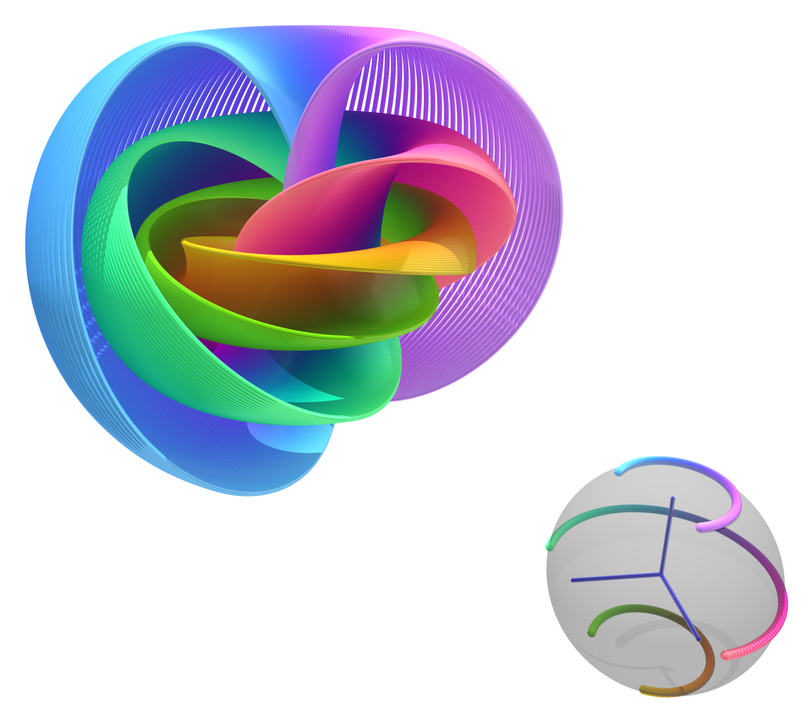
\includegraphics[width=0.5\textwidth]{hopf-fibration.png}
    \caption{The Hopf fibration. Image by Niles Johnson, CC BY-SA 3.0 \url{https://creativecommons.org/licenses/by-sa/3.0}, via Wikimedia Commons.}
    \label{hopf-fig}
\end{figure}
\subsection{Quaternionic projective space $\HP{n}$ and beyond}
The 2-dimensionality of $\mathbb{C}$ ensured that the n-cells of $\CP{n}$ were well spread in dimension, leading to an easy homology calculation. One can wonder if the same method can be applied to the higher dimensional extension of $\mathbb{R}$. Indeed we can! The quaternions $\mathbb{H}$ is a four-dimensional extension of $\mathbb{R}$. It is \textit{not} a field, as it is not commutative. However, it retains all the other requirements of a field, importantly does not have zero-divisors. Rings where every nonzero element has a multiplicative inverse are called \defn{division algebras}. The fact that $\mathbb{H}$ is a division algebra is what allows us to use the same argument as before on the Quaternionic projective space $\HP{n}$.

\begin{prop}
$\HP{n}$ has a cell structure with a $4k$-cell for $0\leq k\leq n$. As a consequence, $$H_k(\HP{n})=\begin{cases}\mathbb{Z} & k=0\text{ mod } 4 , 0\leq k\leq 4n \\ 0 & \text{otherwise}\end{cases}$$
\end{prop}

\begin{proof}
As in previous cases, $\HP{0}=\bullet$, as $z\sim 1$ for every $z\in \mathbb{H}$ by division by $z$. For general $\HP{n}$ we will proceed by induction. $\HP{n}=\mathbb{H}^{n+1}/\sim$
$$(z_1,\dots,z_{n+1})\sim h(z_1,\dots,z_{n+1}), \forall h\in \mathbb{H}$$
If $z_{n+1}\neq 0$, we can divide by $z_{n+1}$ to find a set of unique representations
$$\{(u_1,\dots,u_n,1)\}\homeo \mathbb{H}^n\homeo int(D^{4n})$$
The boundary of this set in $\HP{n}$ is the quotient 
$$\{(z_1,\dots,z_n,0)\}/\sim \homeo \HP{n-1}$$
We can therefore give $\HP{n}$ the CW-structure of $\HP{n-1}$, with an additional $4n$-cell, mapped onto $\HP{n-1}$ via the projection on its boundary $p:S^{4n-1}\rightarrow \HP{n-1}$. By induction, $\HP{n}$ has the CW-structure stated in the proposition. Since $\HP{n}$ has no $m$-cells in adjacent dimensions, its $m$-th homology group is the free abelian group generated by its $m$-cell (or lack thereof).
\end{proof}

\begin{remark}
Notice that $\HP{1}$ has a 0-cell and a 4-cell, and is therefore homeomorphic to $S^{4}$. As in Remark \ref{hopf}, the gluing map of the 8-cell of $\HP{2}$ onto $\HP{1}\iso S^{4}$, therefore gives a "Hopf"-map $S^7\rightarrow S^4$ with the property that the preimage of a point is a "great" copy of $S^3$. If there was a way to keep extending $\mathbb{R}$ to a division algebra for every positive power of two we could repeat this process, yielding "Hopf"-maps from $S^{2^n-1}$ to $S^{n-1}$ for all $n>0$. However, this is false!!! The non-existence of such maps for $n>4$ proves there are no $2^n$-dimensional division algebras of $\mathbb{R}$ for $n>4$.
\end{remark}
\end{document}
